
\section{Cut Continuous Interior Penalty Method for the Biharmonic Problem}%
\label{sec:cutcip_biharmonic_problem}

\subsection{Notation}%
\label{sub:notation}

We will in this report assume $\Omega $ to be a compact and open set in $\mathbb{R} ^{d}$. Let $p \in \mathbb{R} $, $ 1 \le  p \le  \infty$. We define the space $L^{p}\left( \Omega  \right) $ to be the set of all measurable functions $f: \Omega  \mapsto \mathbb{R} $ such that
$\left\lvert f \right\rvert ^{p}$ is Lebesgue measurable, i.e,

\begin{equation*}
    L^{p}\left( \Omega  \right) = \left\{ f: \Omega \mapsto \mathbb{R}  \mid \int_{\Omega }^{} \left\lvert f \right\rvert ^{p} d \Omega  < \infty  \right\}
.\end{equation*}
Let $u \in L^{p}\left( \Omega  \right) $. We define the integral norm of order $p$ to be \[
\| u \|_{ L^{p}\left( \Omega  \right)  }^{  }  = \left( \int_{\Omega }^{} \left\lvert u \right\rvert ^{p} dx  \right) ^{\frac{1}{p}}.
\]
Since $p=2$ is frequently used in this report, we also define for convenience a compact notation $\| u \|_{ \Omega  }^{  }  = \| u \|_{ L^{2}\left( \Omega  \right)  }^{  } $ .  We say that $L^{2}\left( \Omega  \right) $ is a Hilbert space if it is equipped with a inner
product of two functions $u,v \in L^{2}\left( \Omega  \right) $ s.t.
    $
\left( u,v \right) _{\Omega } = \left( u,v \right) _{L^2\left( \Omega  \right) } = \int_{\Omega }^{} u  v dx.
$
We now use this notation for derivatives,
\begin{equation}
\label{eq:mixed_derivative}
\partial ^{\alpha  } f = \frac{\partial ^{\left\lvert \alpha  \right\rvert } f}{ \partial ^{\alpha _{1} } x_{1} \partial ^{\alpha _{2}} x_{2}  }, \quad \text{for } \alpha=\left( \alpha _{1}, \alpha _{2} \right) \text{ and } f \in C^{\left\lvert \alpha  \right\rvert }
\left( \Omega  \right)
.\end{equation}
For $d$ dimensions of order $k$ we define the multi-index $\alpha  = ( \alpha _{1}, \ldots, \alpha _{d})  $ with the absolute value $\abs{ \alpha  } = \sum_{i}^{}  \alpha _{i} = k $ s.t.
\[
\partial ^{\alpha} f = \frac{\partial ^{ \alpha_{1}  }  } {\partial^{} x_{1}^{\alpha _{1}}  } \ldots \frac{\partial ^{ \alpha_{d}  }  } {\partial^{} x_{d}^{\alpha _{d}}  } f
\]

  Let $m\ge 0$ be an integer and let $1 \le  p \le  \infty$ be a real number. Then we define the Sobolev space
\[
H^{m}\left( \Omega  \right) = \left\{ u \in L^{2}\left( \Omega  \right)  \mid  \partial ^{\alpha } u \in L^{2}\left( \Omega  \right)  \forall \alpha : \left\lvert \alpha  \right\rvert  \le m \right\}.
\]
Equipped with the inner product is $H^{m}\left( \Omega  \right) $  denoted as a Hilbert space, that is, for $u,v \in H^{m}\left( \Omega  \right) $, \[
    \left( u,v \right) _{H^{m}\left( \Omega   \right) } = \sum_{\left\lvert \alpha  \right\rvert  \le  m}^{}  \int_{\Omega }^{} \partial ^{\alpha } u \partial ^{\alpha } v dx.
\]
Similarly, the norm is is denoted as,
$
\| u \|_{ H^{m}\left( \Omega  \right)  }^{2  }  =  \| u \|_{ L^{2}\left( \Omega  \right)    }^{2} + \sum_{k = 1}^{m}  \left\lvert u \right\rvert ^{2} _{  H^{k}\left( \Omega  \right) },
$
where the seminorm is defined such that, $ \left\lvert u \right\rvert _{H^{k}( \Omega  ) }^{2} =  \sum_{\left\lvert \alpha  \right\rvert  = k}^{} \| \partial ^{\alpha }u \|_{ \Omega  }^{ 2 }  .
$
We will often denote the shorthand notation $ \| u \|_{ k, \Omega  }^{  } = \| u \|_{ H^{k}( \Omega)  }^{  } $ and $ \abs{ u }_{ k, \Omega  }^{  }  = \abs{ u }_{ H^{k}( \Omega)  }^{  }$.

\subsection{Computational Domains}%
\label{sub:computational_domain}
Assume that $\Omega \subset \mathbb{R} ^{d} $ is a compact set with a boundary  $\Gamma $. In standard FEM methods a key assumption is that the set $\Omega $ is a polyhedra. This is useful since a polyhedra can be fully covered by a collection of polyhedra and, hence, motivating us to define a fitted mesh.
We define a fitted mesh $\mathcal{T} $ of the domain $\Omega $ to be a collection of disjoint polyhedra $\left\{ T \right\}  $ forming a partition of $\Omega $ s.t $\overline{\Omega } = \bigcup _{T \in \mathcal{T} } T $, for illustration see Figure
\ref{fig:domain_mesh}.
Here we say that each $T \in  \mathcal{T} $ is a mesh element or an element.
The mesh size is defined as the maximum diameter $h := h_{max} $ of any polyhedra in the mesh $\mathcal{T} = \left\{ T \right\}  $, that is, $ h_{max} = \max_{T \in \mathcal{T} }  h_{T}$ s.t.
    $h _{T}  = diam\left( T \right)   = \max_{x_1, x_{2} \in T} dist(x_{1}, x_{2})$
Hence, motivating us to use the notation $\mathcal{T} _{h}$ for a mesh $\mathcal{T} $ with size $h$.
 A mesh is conform if $T_{1} \neq T_{2 }$  then $T_{1} \cap T_{2} \neq \emptyset  $ for all $T_{1}, T_{2} \in \mathcal{T}_{h}$. This means that each $T$ share either a vertex or a facet.
Let the chunkiness parameter $c_{T} := h_{T}/r_{T}$, where $r_{T}$  is the largest ball that be inscribed inside a element $T \in \mathcal{T}_{h} $.
A mesh is said to be shape regular if $c_{T}\le  c$ is independent of $T$  and $h$. We also say that the mesh is quasi-uniform only if it is shape regular and $h_{max} \le  c h_{min}$.
In this report will we assume that a mesh $\mathcal{T}_{h} $ is conform, shape regular and quasi-uniform unless specified.
 The fact that the mesh is conform makes is a useful property since the interface between mesh elements has come into contact in the sense
that it is either a vertex or a facet. This with the combination of shape regularity and quasi-uniformity has been a major key to prove important inequalities in broken Sobolev spaces \cite[Chapter 1.4.1]{pietro2012}. Hence, the assumptions are very handy when proving convergence.

 \todo[inline]{ Remove introduction of unfitted mesh until later }
Questions arise when we want to allow for complex geometries where some physical domain $\Omega $ has a smooth boundary $\Gamma $ and, thus, cannot be fully covered of a fitted mesh. This motivates us to define a so-called unfitted mesh.
 Let a background domain $\widetilde{\Omega } \subset \mathbb{R} ^{d} $ have a corresponding mesh $\widetilde{\mathcal{T} _{h}}$.
Assume that the physical domain is the set $\Omega\subset   \widetilde{\Omega }  $ with the corresponding smooth boundary $\Gamma$. We define the unfitted mesh or the active mesh as the triangulation that intersects the interior of $\Omega$, i.e., the intersection $\widetilde{\mathcal{T}_{h} } \cap
 Int(\Omega )     $ where $ Int( \Omega )  = \Omega \setminus \Gamma  $.


Let $\mathcal{T}_{h}  = \left\{ T \right\} $ be a mesh of $\Omega \subset  \mathbb{R} ^d $ consisting of polygons $T \in \mathbb{R} ^{d}$.
The set of all facets is the union of external and internal facets, $\mathcal{F} _{h} = \mathcal{F} ^{ext}_{h} \cup \mathcal{F} _{h}^{int} $, where each are defined like this:
\[
            \mathcal{F}^{int} _{h}  = \left\{ F=T^{+}\cap T^{-}  \mid  T^{+}, T^{-} \in \mathcal{T}_{h}  \right\} \text{ and }
            \mathcal{F}^{ext} _{h}  = \left\{ F= \partial T \cap \partial \Omega    \mid  T  \in \mathcal{T}_{h}  \right\}.
\]
Let $\mathcal{T}_{h} $ be a mesh of $\Omega $ equipped with the facets $\mathcal{F}_{h} $. We will define the following normal vectors
\begin{enumerate}[label=\arabic*)]
    \item We define $n \mid _{T}$ to be unit outward normal on $\partial T$ for each $T \in \mathcal{T}_{h} $
 \item For all $F \in \mathcal{F }^{int} _{h}$ we define $n$ to be the facet normal $ n  \mid_F = n \mid _{T^{+}} $  from $T^{+}$ to $T^{-}$, illustrated in figure \ref{fig:normal}.
 \item For all $F \in F^{ext}_{h}$ we define the facet normal $n \mid _{F} = n \mid _{T} $ to the unit outward normal.
\end{enumerate}
Keep in mind that in many that we often will simply use the notation $n = n \mid _{T}$ in most cases.

    Let $v\in L^2( \Omega ) $ be a scalar function on $\Omega$ with a corresponding shape regular and quasi-uniform mesh $\mathcal{T}_{h} $. We will use the following definitions.
    \begin{enumerate}[label=\arabic*)]
        \item Let $F \in \mathcal{F}^{int} _{h}$ and $v^{\pm}| _{F} = \lim_{t\to 0} v( x \pm tn)   $ for $x \in F$. We define the mean as $\mean{ v} |_{F} = \frac{1}{2} (v^{+}_{F} + v^{-}_{F})   $ and the jump as $\jump{v}|_{F} =  v^{+}_{F} - v^{-}_{F} $.
        \item Let $F \in \mathcal{F}^{ext} _{h}$ and let $ v( x) =  v(x)|_{F} $ for  $x \in F$.
We define the mean as $\mean{ v} |_{F} = v    $ and the jump as $\jump{v}|_{F} = v$.

    \end{enumerate}
    To simplify will we use the notation $\mean{ v } = \mean{ v } \mid _{F}    $ and $\jump{ v } = \jump{ v } \mid _{F}    $ for all $F \in \mathcal{F} _{h}$.
    Remark that if we have to functions $u,v \in L^2( \mathcal{T}_{h} ) $, then the following identity holds $  \jump{ uv }    = \jump{ u }   \mean{ v }    + \mean{ u }  \jump{ v }$.


\begin{figure}[!h]
\centering
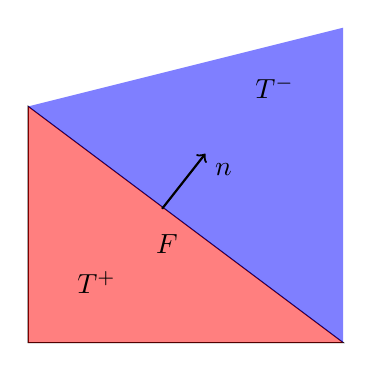
\begin{tikzpicture}[scale=1]
\coordinate (A) at (0,0);
\coordinate (C) at (0,3);
\coordinate (B) at (4,0);
\coordinate (D) at (4,4);
\coordinate (Tm) at (3.5,3.5);
\coordinate (Tp) at (0.5, 0.5);
\coordinate (e) at (1.5, 1.5);
\coordinate (start) at (1.7, 1.7);
\coordinate (end) at (2.25, 2.4);

\draw (A) -- (B) -- (C) -- cycle;
\fill[red, opacity=0.5] (A) -- (B) -- (C);
\fill[blue, opacity=0.5] (B) -- (C) -- (D);
\node[below left] at (Tm) {$T^{-} $ };
\node[above right] at (Tp) {$T^{+}$ };
\node[below right] at (e) {$F$ };

\draw [->, thick] (start) -- (end);
% \node[above right] at (A) {A };
% \node[below right] at (B) {B};
% \node[above right] at (C) {C };
% \node[below right] at (D) {D};
\node[below right] at (end) {$n$};
\end{tikzpicture}

\caption{Facet $F \in \mathcal{F}_h^{int} $ shared by the triangles $T^{+}, T^{-} \in \mathcal{T}_{h} $ and the normal unit vector $n$.  }
    \label{fig:normal}
\end{figure}



\subsection{Broken Sobolev spaces}%
\label{sub:broken_sobolev_spaces}

In this work will we compute norms on discontinuous elements, thus, it will be necessary to define broken Sobolev spaces.

Let $\mathcal{T}_{h} $ be a mesh and some integer $m\le n$. Then we define the broken Sobolev space to be \[
H^{m}( \mathcal{T}_{h} ) := \left\{ v \in L^2( \Omega )  \mid \ v|_{T} \in H^{m}( T) \quad     \forall T \in  \mathcal{T} \right\}
\]
and similarly for the facets $\mathcal{F}_{h} $, that is
\[
    \begin{split}
        L^{2}( \mathcal{F}_{h} ) &:= \left\{ v \in L^2( \mathcal{T}_{h}  )  \mid   \ v|_{F} \in L^{2}( F)  \quad  \forall F \in  \mathcal{F}_{h}   \right\} \\
        H^{m}( \mathcal{F}_{h} ) &:= \left\{ v \in L^2( \mathcal{F}_{h}  )  \mid   \ v|_{F} \in H^{m}( F)  \quad  \forall F \in  \mathcal{F}_{h}   \right\}
    \end{split}
\]
This motivates us to define broken Sobolev norms and inner products using a summation over mesh elements. That is,
\[
 \| v \|_{H^{m}( \mathcal{T}_{h} ) }^{2} = \sum_{T \in  \mathcal{T}_{h} }^{} \| v  \|_{ H^{m}( T ) }^{2  } \quad \text{ and } \quad
 (v ,w )_{H^{m}( \mathcal{T}_{h} ) }^{} = \sum_{T \in \mathcal{T} _{h}}^{} (v ,w )_{ H^{m}( T ) }^{  } .
\]
As expected we use the notation,  $\| v \|_{\mathcal{T}_{h}} =  \| v \|_{L^{2}( \mathcal{T}_{h} ) }$ and  $(v ,w )_{ \mathcal{T}_{h} }^{} = (v ,w )_{L^2( \mathcal{T} ) }^{} $.
That is,
\[
 \| v \|_{H^{m}( \mathcal{F}_{h} ) }^{2} = \sum_{F \in  \mathcal{F}_{h} }^{} \| v  \|_{ H^{m}( F ) }^{2  } \quad \text{ and } \quad
 (v ,w )_{H^{m}( \mathcal{F} ) }^{} = \sum_{T \in \mathcal{F} _{h}}^{} (v ,w )_{ H^{m}( F ) }^{  } .
\]
And again, we often use the more compact notation $\| v \|_{\mathcal{F}_{h}} =  \| v \|_{L^{2}( \mathcal{F}_{h} ) }$ and  $(v ,w )_{ \mathcal{F}_{h} }^{} = (v ,w )_{L^2( \mathcal{F}_{h} ) }^{} $.
A very useful lemma when working on estimates on broken Sobolev spaces is that a if a function is continuous, then the jump between the mesh elements is zero. A function $ v \in  H^{1}( \mathcal{T}_{h} ) $ belongs to $ H^{1}( \Omega )  $ if and only if $ \jump{ v }   = 0, \quad F \in \mathcal{F}^{int}_{h}$.





\subsection{Continuous Interior Penalty Method }%
\label{sub:weak_formulation}





\subsection{Initial discrete formulation}%
\label{sub:initial_discrete_formulation}

Let the $\Omega  \subset \mathbb{R} ^{d} $ be a physical domain with a smooth boundary $\Gamma  $ of class $C^{2}$ .
We want to make a CutFEM version of the CIP problem. Let $\widetilde{\mathcal{T}_{h} } $ be a shape-regular and quasi-uniform background mesh. Let us denote the active set $\mathcal{T} _{h} \subseteq \widetilde{\mathcal{T}}_{h}$ which intersects the interior of the active domain $\Omega $, that is  \[
\mathcal{T} _{h} = \left\{ T \in \widetilde{\mathcal{T} }_{h}  \mid  T \cap (\Omega \setminus \Gamma ) \neq \emptyset    \right\} .
\]
With a corresponding set of interior facets, \[
    \mathcal{F} _{h} = \left\{ F = T^{+} \cap T^{-}  \mid  T^{+}, T^{-} \in \mathcal{T} _{h} \right\},
\]
and a set of cut elements \[
\mathcal{T} _{\Gamma } = \left\{ T \in \mathcal{T} _{h}   \mid  T \cap \Gamma \neq \emptyset  \right\}.
\]
For convenience, will we define also the interior of the active set as $\mathcal{T} _{int}$.
\[
\mathcal{T} _{int} = \left\{ T \in \mathcal{T} _{h}   \mid  T \cap  Int(\Omega ) \neq \emptyset  \right\}.
\]
Hence, we have that the active set is the union of the interior and cut elements, $\mathcal{T} _{h} = \mathcal{T} _{int} \cap \mathcal{T} _{\Gamma }$. For an illustration, see Figure \ref{fig:background_mesh}.


\begin{figure}\centering
\subfloat[]{\label{a}
        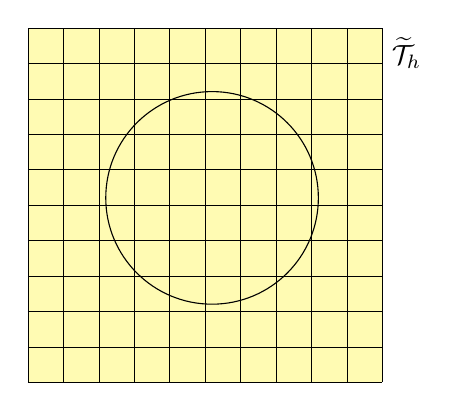
\begin{tikzpicture}[scale=0.9]

            \fill[yellow!30] (-2.5,2.5) -- (2.5,2.5) -- (2.5,-2.5) -- (-2.5,-2.5) -- cycle;

            \draw (0.1, 0.1) circle (1.5cm);
            % Background mesh
            \foreach \i in {-2.5, -2, ..., 2.5} {
                \draw[line width=0.1pt, shift={(-2.5,\i)}] (0,0) -- (5,0);
                \draw[line width=0.1pt, shift={(\i,-2.5)}] (0,0) -- (0,5);
            }


            % Labels
            \node[below right] at (2.5,2.5) {$\widetilde{\mathcal{T}}_{h}$};
        \end{tikzpicture}

}\hfill
\subfloat[]{\label{b}
        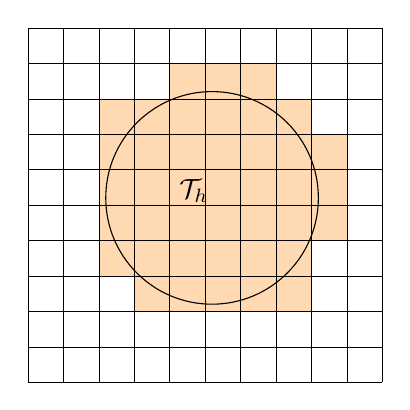
\begin{tikzpicture}[scale=0.9]

            % POTENTIAL ACTIVE MESH
            \fill[orange!30] (2,2) -- (2,-1.5) --(-1.5,-1.5) -- (-1.5,2) -- cycle;

            % ELEMENTS WITH NO INTERSECTION
            % lower left
            \fill[white] (-1.5,-1.5) rectangle (-1.0,-1.0);
            \fill[white] (-1.5,2.0) rectangle (-1.0,1.5);
            \fill[white] (-1.0,2.0) rectangle (-0.5,1.5);
            \fill[white] (2,2) rectangle (1.5,1.5);
            \fill[white] (1.5,2) rectangle (1.0,1.5);
            \fill[white] (2,1.5) rectangle (1.5,1.0);
            \fill[white] (1.5,-1) rectangle (2,-1.5);
            \fill[white] (1.5,-0.5) rectangle (2,-1.0);

            % CUT ELEMENTS
            \fill[orange!30] (-0.5,2.0) rectangle (1.0,1.5);
            \fill[orange!30] (-1.5,1.5) rectangle (0.0,1.0);
            \fill[orange!30] (0.5,1.5) rectangle (1.5,1.0);
            \fill[orange!30] (-1.5,1.0) rectangle (-1.0,-1.0);
            \fill[orange!30] (-1.0,-0.5) rectangle (-0.5,-1.5);
            \fill[orange!30] (-0.5,-1.5) rectangle (1.5,-1.0);
            \fill[orange!30] (1.5,-1) rectangle (1.0,-0.0);
            \fill[orange!30] (1.5,-0.5) rectangle (2.0,1.0);
            \fill[orange!30] (1.0,0.5) rectangle (1.5,1.0);

            \draw (0.1, 0.1) circle (1.5cm);
            % Background mesh
            \foreach \i in {-2.5, -2, ..., 2.5} {
                \draw[line width=0.1pt, shift={(-2.5,\i)}] (0,0) -- (5,0);
                \draw[line width=0.1pt, shift={(\i,-2.5)}] (0,0) -- (0,5);
            }


            % Labels
            % \node[below right] at (2.5,2.5) {$\widetilde{\mathcal{T}}_{h}$};
            % \node[below right] at (0.4,0.5) {$\mathcal{T}_{int}$};
            \node[below right] at (-0.5,0.5) {$\mathcal{T}_{h }$};
        \end{tikzpicture}


}\par

\subfloat[]{\label{c}
        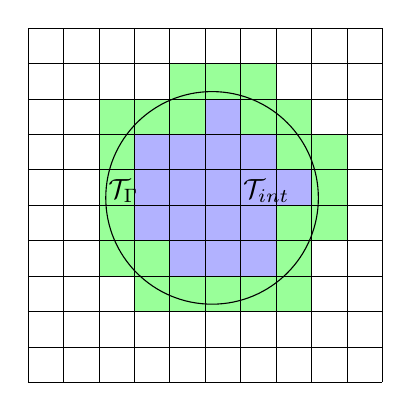
\begin{tikzpicture}[scale=0.9]

            % POTENTIAL ACTIVE MESH
            \fill[blue!30] (2,2) -- (2,-1.5) --(-1.5,-1.5) -- (-1.5,2) -- cycle;

            % ELEMENTS WITH NO INTERSECTION
            % lower left
            \fill[white] (-1.5,-1.5) rectangle (-1.0,-1.0);
            \fill[white] (-1.5,2.0) rectangle (-1.0,1.5);
            \fill[white] (-1.0,2.0) rectangle (-0.5,1.5);
            \fill[white] (2,2) rectangle (1.5,1.5);
            \fill[white] (1.5,2) rectangle (1.0,1.5);
            \fill[white] (2,1.5) rectangle (1.5,1.0);
            \fill[white] (1.5,-1) rectangle (2,-1.5);
            \fill[white] (1.5,-0.5) rectangle (2,-1.0);

            % CUT ELEMENTS
            \fill[green!40] (-0.5,2.0) rectangle (1.0,1.5);
            \fill[green!40] (-1.5,1.5) rectangle (0.0,1.0);
            \fill[green!40] (0.5,1.5) rectangle (1.5,1.0);
            \fill[green!40] (-1.5,1.0) rectangle (-1.0,-1.0);
            \fill[green!40] (-1.0,-0.5) rectangle (-0.5,-1.5);
            \fill[green!40] (-0.5,-1.5) rectangle (1.5,-1.0);
            \fill[green!40] (1.5,-1) rectangle (1.0,-0.0);
            \fill[green!40] (1.5,-0.5) rectangle (2.0,1.0);
            \fill[green!40] (1.0,0.5) rectangle (1.5,1.0);

            \draw (0.1, 0.1) circle (1.5cm);
            % Background mesh
            \foreach \i in {-2.5, -2, ..., 2.5} {
                \draw[line width=0.1pt, shift={(-2.5,\i)}] (0,0) -- (5,0);
                \draw[line width=0.1pt, shift={(\i,-2.5)}] (0,0) -- (0,5);
            }


            % Labels
            \node[below right] at (0.4,0.5) {$\mathcal{T}_{int}$};
            \node[below right] at (-1.5,0.5) {$\mathcal{T}_{\Gamma }$};
        \end{tikzpicture}
}

\caption{Illustration of the background mesh $\widetilde{T}_{h} $, the active set $\mathcal{T} _{h}$, the cut cells $\mathcal{T} _{\Gamma }$ and the interior of the active set $\mathcal{T} _{int}$ }
\label{fig:background_mesh}
\end{figure}

We denote the $C^{0}$ polynomial space of order $k$ as
\[
V_{h} = \left\{ v \in C^{0}\left( \Omega  \right): v_{T} = v | _{T} \in \mathcal{P} ^{k}\left( T \right), \forall T \in
\mathcal{T}_{h}    \right\}
\]

Here we present the CutCIP. The bilinear form $a_{h}:  V_{h}\times  V_{h} \to \mathbb{R} $ and the linear form $l_{h}: V_{h} \to \mathbb{R} $  is defined as,

\begin{equation*}
\begin{split}
a_{h} \left( u, v \right)   =&
    \left( \alpha  u, v \right) _{\Omega }   +  \left( \Delta  u, \Delta v \right) _{\mathcal{T} _{h} \cap \Omega } \\
 & + \left( \mean{  \Delta  u }, \jump{ \partial _{n }v} \right)_{\mathcal{F}_{h} \cap \Omega  }  + \left( \mean{ \Delta  v }, \jump{ \partial _{n}u }      \right)_{\mathcal{F}_{h} \cap \Omega }  + \frac{\gamma }{h}  \left( \jump{ \partial _{n} u}, \jump{ \partial _{n} v   }   \right)_{\mathcal{F}_{h}\cap \Omega } \\
 & + \left(   \Delta  u ,  \partial _{n }v \right)_{\Gamma   }  + \left(  \Delta  v ,  \partial _{n}u       \right)_{\Gamma  }  + \frac{\gamma }{h}  \left(  \partial _{n} u,  \partial _{n} v      \right)_{ \Gamma } \\
 l_{h}( v_{h}) & =  \left( f, v \right) _{\Omega } - ( g_{2},  v )_{\Gamma } -  ( g_{1}, \Delta  v  )_{\Gamma }  + \frac{\gamma }{h} ( g_{2}, \partial _{n} v  )_{\Gamma }
\end{split}
\end{equation*}

\todo[inline]{ Do the derivation. See \cite{georgoulis2009discontinuous}. }
\red{
\begin{equation}
\begin{split}
a_{h} \left( u, v \right)   =&   \left( \alpha  u, v \right) _{\mathcal{T} _{h} \cap \Omega }   +  \left( D^2 u, D^2v \right) _{\mathcal{T} _{h} \cap \Omega} \\
 & +
  \left( \mean{  \partial _{n n} u }, \jump{ \partial _{n }v} \right)_{\mathcal{F}_{h}^{} \cap \Omega}  +
 \left( \mean{ \partial _{n n} v }, \jump{ \partial _{n}u }      \right)_{\mathcal{F}_{h}^{} \cap \Omega} \\
 & + ( \partial _{nn} u, \partial _{n} v)_{\Gamma } + ( \partial _{nn} v, \partial _{n} u)_{\Gamma }
 \\
 & + \frac{\gamma }{h}  \left( \jump{ \partial _{n} u}, \jump{ \partial _{n} v_{}   }   \right)_{\mathcal{F}_{h}^{} \cap \Omega} +  \frac{\gamma }{h}  \left(  \partial _{n} u,  \partial _{n} v_{}      \right)_{\Gamma } \\
\end{split}
.
\end{equation}
 \[
l_{h}( v) =  ( f,v)_{\mathcal{T} _{h} \cap \Omega } - (g_{2},v) - ( g_{1}, \partial _{nn}v) _{\Gamma } + \frac{\gamma }{h}  ( g_{1}, \partial _{n} v)   .
\]
}
Similarly the linear form is defined as
 \[
l_{h}( v) =  ( f,v)_{\mathcal{T} _{h} \cap \Omega } - (g_{2},v) - ( g_{1}, \partial _{nn}v) _{\Gamma } + \frac{\gamma }{h}  ( g_{1}, \partial _{n} v)   .
\]


To make sure the problem is stabilized will we add ghost-penalty $g_{h}: V_{h} \times  V_{h} \to \mathbb{R} $. That is, we define the discrete problem to find a $u \in V_{h}$ s.t. \[
A_{h}( u ,v ) := a_{h}( u, v)  + g_{h}( u,v) = l_{h} ( v) \quad  \forall v \in  V_{h}.
\]

Keep in mind that in contrast to the standard CIP methods, this method is defined on an unfitted mesh. As we will see, the analysis is the ghost penalty a method to ensure numerical stability on cut cell $\mathcal{T} _{\Gamma }$. The main reason why
this numerical instability is happening for a unfitted mesh is that when a cell is badly cut, see examples in Figure \ref{fig:intersection-example}.
In other words, when a cell is "badly cut," it means that it is intersected by the boundary $\Gamma$ in such a way that only a very small part of the cell lies inside or outside the domain. This can lead to a very poor condition number of the local system matrix corresponding to such a cell, causing numerical instability.

The ghost penalty stabilization technique is designed to tackle this issue. Essentially, this approach introduces additional terms into the finite element method that penalize jumps in the discrete solution and its gradients across cell interfaces,
typically the cut-cells. This penalty not only improves the conditioning of the system matrix, but also enhances the robustness of the method with respect to the location of the boundary inside each cell. However, to make this possible is to assume a
so-called fat-intersection property which will be relevant in section \textbf{TODO: Add section to ghost penalty}.

\begin{figure}[htbp]
    \centering
    \begin{minipage}{0.4\textwidth}
        \centering
        \begin{tikzpicture}
            \coordinate (center) at (0, 0);

            % Reference hexagon vertices
            \coordinate (A1) at (0:2.5);
            \coordinate (A2) at (60:2.5);
            \coordinate (A3) at (120:2.5);
            \coordinate (A4) at (180:2.5);
            \coordinate (A5) at (240:2.5);
            \coordinate (A6) at (300:2.5);
            \coordinate (A7) at (300:2.5);


            \fill[green!40] (center) --(A1) -- (A2) -- (A3) -- (A4) -- (A5)  -- cycle;
            \fill[blue!30] (center) -- (A5)--(A6)-- (A7) -- (A1) -- cycle;

            % Draw the individual edges
            \draw (center) -- (A1);
            \draw (center) -- (A2) --(A1);
            \draw (center) -- (A3);
            \draw (center) -- (A4);
            \draw (A2) -- (A3);
            \draw (A3) -- (A4);
            \draw (A5) -- (A6);
            \draw (A4) -- (A5);
            \draw (center) -- (A5);
            \draw (center) -- (A6) -- (A1);

            \coordinate (Ti) at (-0,-1.5);
            \coordinate (Tg) at (0.5,2.2);
            \node[below] at (Tg) {$\mathcal{T}_{\Gamma }$};
            \node[below] at (Ti) {$\mathcal{T}_{int }$};

            \coordinate (T0) at (-0,1.2);
            \coordinate (T1) at (-1.1,-0.4);
            % \node[below] at (T0) {$T$};
            % \node[below] at (T1) {$T'$};

            \coordinate (C1) at (-3,-1.0);
            \coordinate (C2) at (2.6,0.2);
            \draw[-, line width=2pt, >=stealth] ($(C2)$) to[bend right=16.9] node[midway,xshift=-2.3cm, yshift=-1.3cm] {$\Gamma $} ($(C1)$);


        \end{tikzpicture}
    \end{minipage}
    \hspace{1cm}
    \begin{minipage}{0.4\textwidth}
        \centering
        \begin{tikzpicture}
            \coordinate (center) at (0, 0);

            % Reference hexagon vertices
            \coordinate (A1) at (0:2.5);
            \coordinate (A2) at (60:2.5);
            \coordinate (A3) at (120:2.5);
            \coordinate (A4) at (180:2.5);
            \coordinate (A5) at (240:2.5);
            \coordinate (A6) at (300:2.5);
            \coordinate (A7) at (300:2.5);


            \fill[green!40] (center) --(A1) -- (A2) -- (A3) -- (A4) -- cycle;
            \fill[blue!30] (center) (A4) -- (A5)--(A6)-- (A7) -- (A1) -- cycle;

            % Draw the individual edges
            \draw (center) -- (A1);
            \draw (center) -- (A2) --(A1);
            \draw (center) -- (A3);
            \draw (center) -- (A4);
            \draw (A2) -- (A3);
            \draw (A3) -- (A4);
            \draw (A5) -- (A6);
            \draw (A4) -- (A5);
            \draw (center) -- (A5);
            \draw (center) -- (A6) -- (A1);

            \coordinate (Ti) at (-0,-1.5);
            \coordinate (Tg) at (0.5,2.2);
            \node[below] at (Tg) {$\mathcal{T}_{\Gamma }$};
            \node[below] at (Ti) {$\mathcal{T}_{int }$};

            \coordinate (T0) at (-0,1.2);
            \coordinate (T1) at (-1.1,-0.4);
            \node[below] at (T0) {$T$};

            \coordinate (C1) at (-3,0.1);
            \coordinate (C2) at (2.6,0.2);
            \draw[-, line width=2pt, >=stealth] ($(C2)$) to[bend right=0.9] node[midway,xshift=-2.5cm, yshift=-0.5cm] {$\Gamma $} ($(C1)$);

        \end{tikzpicture}
    \end{minipage}
        \caption{Two examples of bad cut cells. At some point it is even hard to distinguish between interior and cut cells.}
        \label{fig:intersection-example}
\end{figure}

We define the underlying norms for $ v \in V_{h} $ as
    \begin{align}
        \label{eq:bi_ah_norm}
        \| v \|_{ a_{h} }^{ 2 } & =    \alpha  \|   v \|_{ \mathcal{T} _{h} \cap \Omega  }^{ 2}  + \|  \Delta v \|_{\mathcal{T} _{h} \cap \Omega   }^{ 2 } + \gamma \| h^{-\frac{1}{2}} \jump{ \partial _{n} v }   \|_{ \mathcal{F}_{h}^{}\cap \Omega    }^{ 2
        } + \gamma \| h^{-\frac{1}{2}}  \partial _{n} v    \|_{ \Gamma   }^{ 2 },    \\
        \label{eq:bi_gh_norm}
\abs{ v } _{g_{h}}^{2} & = g( v,v) \\
        \label{eq:bi_Ah_norm}
\| v \|_{A_{h}  }^{  2}  & = \| v \|_{ a_{h} }^{ 2 } + \abs{ v } _{g_{h}}^{2}
    \end{align}

    \red{
    \[
        \| v \|_{ a_{h} }^{ 2 }  =   \alpha \|   v \|_{ \mathcal{T} _{h} \cap \Omega  }^{ 2}  + \| D^2 v \|_{\mathcal{T} _{h} \cap \Omega   }^{ 2 } + \gamma \| h^{-\frac{1}{2}} \jump{ \partial _{n} v }   \|_{ \mathcal{F}_{h}^{}\cap \Omega    }^{ 2 }
        + \gamma \| h^{-\frac{1}{2}}  \partial _{n} v    \|_{ \Gamma   }^{ 2 }, \\
    \]
}
and for $v \in V + V_{h}$ we get, \[
    \begin{split}
\| v \|_{ a_{h}, * }^{  2} & =\| v \|_{ a_{h} }^{ 2 } +  \| h^{\frac{1}{2}} \mean{ \Delta  v }   \|_{\mathcal{F} _{h}^{} \cap \Omega   }^{  2} +  \| h^{\frac{1}{2}} \Delta  v    \|_{ \Gamma }^{  2}  \\
\| v \|_{A_{h},*  }^{  2}  & = \| v \|_{ a_{h},* }^{ 2 } + \abs{ v } _{g_{h}}^{2}
    \end{split}
\]
\red{
\[
    \begin{split}
\| v \|_{ a_{h}, * }^{  2} & =\| v \|_{ a_{h} }^{ 2 } +  \| h^{\frac{1}{2}} \mean{ \partial _{nn} v }   \|_{\mathcal{F} _{h}^{} \cap \Omega   }^{  2} +  \| h^{\frac{1}{2}} \partial _{nn} v    \|_{ \Gamma }^{  2}  \\
    \end{split}
\]
}
\begin{remark}
Note that it holds that $\mathcal{T} _{h} \cap  \Omega   = \Omega  $ and $\mathcal{T} _{h} \cap  \Gamma  = \Gamma $. Depending on context, we choose the best suitable notation.
\end{remark}

\subsection{Stability estimate}%
\label{sub:stability_estimate}

\begin{figure}[htbp]
  \centering

    \begin{tikzpicture}
        \coordinate (center) at (0, 0);

        % Reference hexagon vertices
        \coordinate (A1) at (0:2.5);
        \coordinate (A2) at (60:2.5);
        \coordinate (A3) at (120:2.5);
        \coordinate (A4) at (180:2.5);
        \coordinate (A5) at (240:2.5);
        \coordinate (A6) at (300:2.5);
        \coordinate (A7) at (300:2.5);


        \fill[green!40] (center) --(A1) -- (A2) -- (A3) -- (A4) -- (A5)  -- cycle;
        \fill[blue!30] (center) -- (A5)--(A6)-- (A7) -- (A1) -- cycle;

        % Draw the individual edges
        \draw[dotted, line width=1.5pt] (center) -- (A1);
        \draw[dotted, line width=1.5pt] (center) -- (A2) --(A1);
        \draw[dotted, line width=1.5pt] (center) -- (A3);
        \draw[dotted, line width=1.5pt] (center) -- (A4);
        \draw (A2) -- (A3);
        \draw (A3) -- (A4);
        \draw (A5) -- (A6);
        \draw[dotted, line width=1.5pt] (A4) -- (A5);
        \draw[dotted, line width=1.5pt] (center) -- (A5);
        \draw (center) -- (A6) -- (A1);

        \coordinate (Ti) at (-0,-1.5);
        \coordinate (Tg) at (0.5,2.2);
        \node[below] at (Tg) {$\mathcal{T}_{\Gamma }$};
        \node[below] at (Ti) {$\mathcal{T}_{int }$};

        \coordinate (T0) at (-0,1.2);
        \coordinate (T1) at (-1.1,-0.4);
        \node[below] at (T0) {$T$};
        \node[below] at (T1) {$T'$};

        \coordinate (C1) at (-3,-1.0);
        \coordinate (C2) at (2.6,0.2);
        \draw[-, line width=2pt, >=stealth] ($(C2)$) to[bend right=16.9] node[midway,xshift=-2.3cm, yshift=-1.3cm] {$\Gamma $} ($(C1)$);


\end{tikzpicture}

  \caption{
        For $T \in \mathcal{T}_{\Gamma}$ there is a patch $P$ of $\text{diam} P \lesssim h$ which contains $T$ and an element $T^{\prime}$ with a fat intersection satisfying
        $ \left|T^{\prime} \cap \Omega\right|_d \geqslant c_s\left|T^{\prime}\right|_d $
        for some mesh independent $c_s>0$. Here the dotted lines is illustration  $\mathcal{F}_{h}^{g} $.
}
  \label{fig:fat-intersection-property}
\end{figure}

Similarly for the Poisson problem will we have the following assumptions for the computational mesh;

\begin{enumerate}[label=\textbf{S.\arabic*}]
    \item\label{as:s1} Boundary $\Gamma $ is of $C^2$
    \item\label{as:s2} The mesh $\mathcal{T} _{h}$ is quasi-uniform.
    \item \label{as:s3}For a $T \in \mathcal{T} _{\Gamma }$ there exists a path $P$ of $diam(P) \lesssim h$ which contains $T$ and an element $T'$ with a so-called fat intersection $
    \abs{ T' \cap \Omega  } _{d} \ge \abs{ T' } _{d}$.
\end{enumerate}

\red{
From basic theory we have the following inverse estimate for $ v \in \mathcal{P}^{k}( T)$ s.t. \[
     \| \partial _{nn}  v \|_{F   }^{ }  \lesssim  \| h_{T}^{-\frac{1}{2}} D ^2 v \|_{ T }^{  },
\]
where the hidden constant depend on dimension $d$, order $k$ and the shape regularity. Similarly for cut elements is it easy to see that this must hold,
\begin{equation*}
     \| \partial _{nn}  v \|_{F \cap \Omega    }^{  }  \lesssim\| \partial _{nn}  v \|_{F }^{  }  \lesssim   \| h_{T}^{-\frac{1}{2}} D ^2 v \|_{ T }^{  }.
\end{equation*}
A useful variant is the following inequality that is,
\begin{equation*}
\| \partial _{nn} v \|_{ \Gamma \cap T  }^{  } \lesssim h^{-\frac{1}{2}} \| D^2 v \|_{ T }^{  }.
\end{equation*}
Summation the inverse inequalities over $\mathcal{F}_{h} $ and $\mathcal{T}_{h} $ implies that
\begin{align}
\label{eq:bi_cut_inverse_1}
\| \partial _{nn} v \|_{ \mathcal{T} _{h} \cap \Gamma  }^{  } &\lesssim h^{-\frac{1}{2}} \| D^2 v \|_{ \mathcal{T}_h }^{  }, \\
\label{eq:bi_cut_inverse_2}
\| \partial _{nn}  v \|_{ \mathcal{F}_h \cap \Omega    }^{  }  &  \lesssim   h^{-\frac{1}{2}} \| D^2 v \|_{ \mathcal{T}_h  }^{  }.
\end{align}
In fact, combining the inequalities we get the identity,
\begin{equation}
\label{eq:bi_identity}
h\| \partial _{nn}  v \|_{ \mathcal{F}_h \cap \Omega    }^{2 } + h\| \partial _{nn} v \|_{ \mathcal{T} _{h} \cap \Gamma  }^{2  } \lesssim \| D^2 v \|_{ \mathcal{T} _{h}  }^{2  }.
\end{equation}
}

We may introduce our first assumption on the ghost penalty.
\begin{assumption}[EP1]
    \label{as:bi_EP1}
    The ghost penalty $g_{h}$ extends the $H^{1}$ norm s.t. \[
    \| \Delta  v \|_{ \mathcal{T} _{h} }^{ 2 } \lesssim  \| \Delta  v \|_{ \Omega  }^{ 2 } + \abs{ v } _{g_{h}}^{2}.
    \]
    \red{
    The ghost penalty $g_{h}$ extends the $H^{1}$ norm s.t. \[
    \| D^2 v \|_{ \mathcal{T} _{h} }^{ 2 } \lesssim  \| D^2 v \|_{ \Omega  }^{ 2 } + \abs{ v } _{g_{h}}^{2}.
    \]
}
\end{assumption}
Combing the results we get the following convenient corollary.

\begin{corollary}
    \label{cor:bi_inverse_thm}
    Let $g_{h}$ satisfy Assumption \ref{as:bi_EP1} then
    \[
            h\| \partial _{nn}  v \|_{ \mathcal{F}_h^{} \cap \Omega    }^{2 } + h\| \partial _{nn} v \|_{ \mathcal{T} _{h} \cap \Gamma  }^{2  }   \lesssim  \| D^2 v \|_{ \Omega  }^{ 2 } + \abs{ v } _{g_{h}}^{2} \\
              \lesssim \| v \|_{ A_{h} }^{  2}
    \]
\end{corollary}
\begin{proof}
    The first inequality is a direct result of \eqref{eq:bi_identity} and Assumption \ref{as:bi_EP1}. The second inequality is simply a results of the definition \eqref{eq:bi_Ah_norm}.
\end{proof}

\begin{lemma}
    \label{lemma:bi_Ah_coercive}
    The discrete form $A_{h}$ is coercive, that is, \[
    \| v \|_{ A_{h} }^{ 2 }  \lesssim A_{h}( v,v) \forall v \in V_{h}
    \]
\end{lemma}


\begin{proof}
    Let $v \in V^{h}$.
    Observe that \[
    A_{h}( v,v) = a_{h}( v,v)  + \abs{ v }_{g_{h}}^{2}
    \]
    Thus, since the second term already is part of the $\| \cdot  \|_{ A_{h} }^{  } $ norm is a good start to focus on the $a_{h}$ term, that is,
    \[
    \begin{split}
       a_{h}( v,v) &=   \|\ |\alpha|^{\frac{1}{2}} \cdot v  \|_{   \Omega   }^{2} + \| D^2v \|_{   \Omega  }^{2  } + 2 ( \mean{ \partial _{nn} v }, \jump{ \partial _{n} v }    )_{\mathcal{F} ^{}_{h} \cap \Omega }  + 2 (  \partial _{nn} v ,
       \partial _{n} v  )_{\Gamma } \\
                   & \quad+ \frac{\gamma }{h}  \|  \jump{ \partial _{n} v }\|_{\mathcal{F} _{h}^{}  }^{ 2 } + \frac{\gamma }{h}  \| \partial _{n} v \|_{ \Gamma  }^{ 2 }
    \end{split}
    \]
    We will first focus on the symmetry terms. Using Cauchy-Schwarz we observe that \[
        \begin{split}
    ( \mean{ \partial _{nn} v }  , \jump{ \partial _{n} v }  )_{\mathcal{F}^{}_{h}\cap \Omega  } & \ge - \| h^{\frac{1}{2}}\mean{ \partial _{nn} v }   \|_{ \mathcal{F}^{}_{h}\cap \Omega   }^{  }  \|h^{-\frac{1}{2}} \jump{ \partial _{n} v }   \|_{
    \mathcal{F}^{}_{h}\cap \Omega   }^{  } \\
    (  \partial _{nn} v   ,  \partial _{n} v   )_{\Gamma   } & \ge - \| h^{\frac{1}{2}} \partial _{nn} v    \|_{ \Gamma    }^{  }  \|h^{-\frac{1}{2}}  \partial _{n} v    \|_{ \Gamma    }^{  }
        \end{split}
    \]
    Using inverse-inequalities \eqref{eq:bi_cut_inverse_1} and \eqref{eq:bi_cut_inverse_2} and the Corollary \ref{cor:bi_inverse_thm} can we easily observe that \[
        \begin{split}
     \| \mean{ \partial _{nn}v } \|_{ \mathcal{T}_{h} \cap \Omega    }^{  2} & \le C_{1} \| D^2 v \|_{ \mathcal{T}_{h}   }^{2  } \le  C  (\| D^2 v \|_{ \Omega  }^{ 2 }  + \abs{ v } _{ g_{h} }^{2  } )  \\
     \|  \partial _{nn}v  \|_{ \Gamma     }^{ 2 } & \le C_{2} \| D^2 v \|_{ \mathcal{T} _{h}  }^{2  } \le C  (\| D^2 v \|_{ \Omega  }^{ 2 }  + \abs{ v } _{ g_{h} }^{2  } )
        \end{split}
    \]
    Thus, by applying Youngs $\varepsilon $-inequality, $2ab \le  \varepsilon^{-1} a^{2} + \varepsilon b^{2} $, is it natural to see that,
    \[
        \begin{split}
- C_{1}^{\frac{1}{2}} \| D^2 v    \|_{ \mathcal{T} _{h}   }^{  }  \|h^{-\frac{1}{2}} \jump{ \partial _{n} v }   \|_{ \mathcal{F}^{}_{h}\cap \Omega   }^{  }
& \ge - \frac{1}{\varepsilon } C  (\| D^2 v \|_{ \Omega  }^{ 2 }  + \abs{ v } _{ g_{h} }^{2  } ) -  \varepsilon \|h^{-\frac{1}{2}} \jump{ \partial _{n} v }   \|_{ \mathcal{F}^{}_{h}\cap \Omega   }^{2  } \\
- C_{2}^{\frac{1}{2}}  \| D^2 v \|_{ \mathcal{T} _{h} }^{  } \| h^{-\frac{1}{2}}  \partial _{n} v    \|_{ \Gamma    }^{  }
& \ge - \frac{1}{\varepsilon } C  (\| D^2 v \|_{ \Omega  }^{ 2 }  + \abs{ v } _{ g_{h} }^{2  } ) -  \varepsilon \|h^{-\frac{1}{2}}  \partial _{n} v    \|_{ \Gamma    }^{2  } \\
        \end{split}
    \]
    Combining these ideas do we end up with the following inequality,
    \[
    \begin{split}
       a_{h}( v,v)  \ge& \     \|\ |\alpha|^{\frac{1}{2}} \  v  \|_{   \Omega   }^{2} +\| D^2v  \|_{   \Omega   }^{2} -  \frac{1}{\varepsilon } 4C  (\| D^2 v \|_{ \Omega  }^{ 2 }  + \abs{ v } _{ g_{h} }^{2  } )  \\
                       & + (\gamma - 2\varepsilon  )\left( \|h^{-\frac{1}{2}}  \jump{ \partial _{n} v }\|_{\mathcal{F} _{h}^{} \cap \Omega   }^{ 2 } + \| h^{-\frac{1}{2}} \partial _{n} v \|_{ \Gamma  }^{ 2} \right)        \\
    \end{split}
    \]
    This inequality is useful, since if we apply it on the $\| \cdot  \|_{ A_{h} }^{  } $ we have a extra ghost penalty term s.t.,

    \[
        \begin{split}
     A_{h}( v,v) & = a( v,v) + \abs{ v }_{g_{h}}^{2} \\
     &\ge  \   \| \ |\alpha|^{\frac{1}{2}} \  v  \|_{   \Omega   }^{2} + (1  - \frac{1}{\varepsilon } 4C)  (\| D^2 v \|_{ \Omega  }^{ 2 }  + \abs{ v } _{ g_{h} }^{2  } )  \\
                       & + (\gamma - 2\varepsilon  )\left( \|h^{-\frac{1}{2}}  \jump{ \partial _{n} v }\|_{\mathcal{F} _{h}^{}\cap \Omega   }^{ 2 } + \| h^{-\frac{1}{2}} \partial _{n} v \|_{ \Gamma  }^{ 2} \right)        .
        \end{split}
    \]
    Setting $\varepsilon = 8C$ and $C=\frac{\gamma }{32} $ we simplify the problem to \[
        \begin{split}
           A_{h}( v,v)  \ge& \   \| \ |\alpha|^{\frac{1}{2}} \    v  \|_{  \Omega   }^{2} + \frac{1}{2}  (\| D^2 v \|_{ \Omega  }^{ 2 }  + \abs{ v } _{ g_{h} }^{2  } )  \\
                       & + \frac{\gamma }{2}\left( \|h^{-\frac{1}{2}}  \jump{ \partial _{n} v }\|_{\mathcal{F} _{h}^{}\cap \Omega   }^{ 2 } + \| h^{-\frac{1}{2}} \partial _{n} v \|_{ \Gamma  }^{ 2} \right) \\
                        \gtrsim & \  \| v \|_{ A_{h} }^{2  }
        \end{split}
    \]
    Hence, proof is complete.
\end{proof}

\begin{lemma}
    \label{lemma:bi_Ah_bounded}
    The discrete form $A_{h}$ is bounded, that is,
    \begin{equation}
    \label{eq:bi_A_h_bounded}
     A_{h}( v,w) \lesssim \| v \|_{A_{h}  }^{  }\| v \|_{A_{h}  }^{  }  \forall w \in V_{h}
    \end{equation}
    Moreover, for $v \in V_{h} + V$  and $w \in V_{h}$ the discrete form $a_{h}$ satisfies
    \begin{equation}
        \label{eq:bi_a_h_bounded}
        a_{h} ( v,w) \lesssim \| v \|_{ a_{h},* }^{  } \| w \|_{ A_{h} }^{  }
    \end{equation}
\end{lemma}

\begin{proof}
    We will divide the proof in two steps.
    \begin{enumerate}[label=\arabic*)]
        \item The goal is to prove the inequality \eqref{eq:bi_A_h_bounded}. \[
                \abs{ A_{h}( v ,w ) } \lesssim   \abs{a_{h}( v, w) }   + \abs{g_{h}( v,w)  }          \]
                By assumption is the ghost penalty $g_{h}$ positive semi-definite, thus, it fulfills the Cauchy-Schwartz inequality \[
                \abs{ g_{h}(v,w ) } \lesssim \abs{ v } _{g_{h}}\abs{ w }_{g_{h}}
                \]
                Hence, by definition is $\abs{ g_{h}(v,w ) } \lesssim \| v \|_{ A_{h} }^{  } \| w \|_{ A_{h} }^{  } $. Now it remains to show that the bilinear term $ a_{h}$ is bounded.
                \begin{equation}
                    \begin{split}
                        \abs{ a_{h} \left( v, w \right) }   \le  &   \abs{\left( \alpha  v, w \right) _{\mathcal{T} _{h} \cap \Omega }  }    +  \abs{\left( D^2 v, D^2w \right) _{\mathcal{T} _{h} \cap \Omega}  }  \\
                                                     & + \abs{\left( \mean{  \partial _{n n} v }, \jump{ \partial _{n }w} \right)_{\mathcal{F}_{h}^{} \cap \Omega}  }   +
                                                     \abs{\left( \mean{ \partial _{nn } v }, \jump{ \partial _{n}w }      \right)_{\mathcal{F}_{h}^{} \cap \Omega}  } \\
                                                     & + \abs{\left(  \partial _{n n} v ,  \partial _{n }w \right)_{\Gamma }}     +
                                                     \abs{\left(  \partial _{n n} w ,  \partial _{n}v       \right)_{\Gamma }  }
                                                     \\
                                                     & + \frac{\gamma }{h} \abs{ \left( \jump{ \partial _{n} v}, \jump{ \partial _{n} w   }   \right)_{\mathcal{F}_{h}^{} \cap \Omega}  } + \frac{\gamma }{h} \abs{ \left(  \partial _{n} v,  \partial _{n} w
                                                     \right)_{\Gamma }  }
                    \end{split}
                \end{equation}
                The strategy is to bound each term individually using Cauchy-Schwartz. We can easily see that $\abs{\left( \alpha  v, w \right) _{\mathcal{T} _{h} \cap \Omega }  }   \lesssim \| v \|_{a_{h}  }^{  } \| w \|_{ a_{h} }^{  } $ and that
                $\abs{\left( D^2 v, D^2w \right) _{\mathcal{T} _{h} \cap \Omega}  } \lesssim \| v \|_{a_{h}  }^{  } \| w \|_{ a_{h} }^{  } $ using Cauchy Schwartz. For the symmetric terms we also apply the inverse inequality
                \eqref{eq:bi_cut_inverse_2}.
                \[
                    \begin{split}
                    \abs{\left( \mean{ \partial _{n n} v }, \jump{ \partial _{n}w }      \right)_{\mathcal{F}_{h}^{} \cap \Omega}  } & \lesssim  \|\mean{ \partial _{n n} v }  \|_{ \mathcal{F}_{h}^{} \cap \Omega}^{  }\|\jump{ \partial _{n} w }  \|_{
                    \mathcal{F}_{h}^{} \cap \Omega}^{  } \\
                    & \lesssim  \|h^{\frac{1}{2}} \partial _{n n} v  \|_{ \mathcal{F}_{h}^{} \cap \Omega}^{  }\| h^{-\frac{1}{2}} \jump{ \partial _{n} w }     \|_{\mathcal{F}_{h}^{} \cap \Omega}^{  } \\
                    & \lesssim  \| v \|_{A_{h}  }^{  } \|w    \|_{ a_{h}}^{  }
                    \end{split}
                \]
                Here we used the Corollary \ref{cor:bi_inverse_thm} s.t.  $\|h^{\frac{1}{2}} \partial _{n n}  v \|_{\mathcal{F}_{h}^{} \cap \Omega} \lesssim \| v \|_{ A_{h}  }^{  }  $.
              The boundedness interior penalty  inequality is showed in this manner, \[
             \frac{\gamma }{h} \abs{ \left( \jump{ \partial _{n} v}, \jump{ \partial _{n} w   }   \right)_{\mathcal{F}_{h}^{} \cap \Omega}  }  \lesssim  \|h^{-\frac{1}{2}} \jump{ \partial _{n} v}  \|_{ \mathcal{F}_{h}^{} \cap \Omega }^{  }
             \|h^{-\frac{1}{2}} \jump{ \partial _{n} w}  \|_{ \mathcal{F}_{h}^{} \cap \Omega }^{  }  \lesssim  \| v  \|_{ a_{h} }^{  }
             \| w  \|_{ a_{h} }^{  }.
             \]
              Now it remains to handle boundary terms. \[
                \abs{ ( \partial _{nn} v, \partial _{n} w)_{\Gamma } }  \lesssim \| h^{\frac{1}{2}}\partial _{nn} v \|_{\Gamma   }^{  } \| h^{-\frac{1}{2}} \partial _{n}w \|_{\Gamma   }^{  }  \lesssim \|  v \|_{A_{h}  }^{  } \| w \|_{ a_{h}   }^{  }
             \]
             Again, here we used the Corollary \ref{cor:bi_inverse_thm}.
             Finally, using the definition of the norm is it easily to see that,
             \[
\frac{\gamma }{h} \abs{ \left(  \partial _{n} v,  \partial _{n} w \right)_{\Gamma }  } \lesssim \gamma  \| h^{-\frac{1}{2}} \partial _{n} v \|_{  \Gamma }^{  } \| h^{-\frac{1}{2}} \partial _{n} w \|_{\Gamma   }^{  } \lesssim \| v \|_{ a_{h} }^{  }
\| w \|_{ a_{h} }^{  } .
             \]

             Obviously is $\| v \|_{a_{h}  }^{  } \lesssim \| v \|_{A_{h}  }^{  }$. Hence, we have showed that all terms in $a_{h}$ is bounded in the $\|\cdot   \|_{A_{h}  }^{  } $ norm.
         \item The goal is to prove \eqref{eq:bi_a_h_bounded} using many of the same ideas as in the first part. Let $v \in V_{h} +V $ and $v \in V_{h}$. Next step is to show that the bilinear term $ a_{h}$ is bounded.
                \begin{equation}
                    \begin{split}
                        \abs{ a_{h} \left( v, w \right) }   \le  &   \abs{\left( \alpha  v, w \right) _{\mathcal{T} _{h} \cap \Omega }  }    +  \abs{\left( D^2 v, D^2w \right) _{\mathcal{T} _{h} \cap \Omega}  }  \\
                                                     & + \abs{\left( \mean{  \partial _{n n} v }, \jump{ \partial _{n }w} \right)_{\mathcal{F}_{h}^{} \cap \Omega}  }   + \abs{\left( \mean{ \partial _{nn } w }, \jump{ \partial _{n}v }
                                                     \right)_{\mathcal{F}_{h}^{} \cap \Omega}  } \\
                                                     & + \abs{\left(  \partial _{n n} v ,  \partial _{n }w \right)_{\Gamma }}     +
                                                     \abs{\left(  \partial _{n n} w ,  \partial _{n}v       \right)_{\Gamma }  }
                                                     \\
                                                     & + \frac{\gamma }{h} \abs{ \left( \jump{ \partial _{n} v}, \jump{ \partial _{n} w   }   \right)_{\mathcal{F}_{h}^{} \cap \Omega}  } + \frac{\gamma }{h} \abs{ \left(  \partial _{n} v,  \partial _{n} w
                                                     \right)_{\Gamma }  }
                    \end{split}
                \end{equation}
                     We can easily observe from the first part that this must holds, \[
    \abs{\left( \alpha  v, w \right) _{\mathcal{T} _{h} \cap \Omega }  }    +  \abs{\left( D^2 v, D^2w \right) _{\mathcal{T} _{h} \cap \Omega}  } \lesssim \| v \|_{ a_{h},* }^{  } \| w \|_{A_{h}  }^{  }.
    \]
    And for the symmetric interior terms,
    \[
        \begin{split}
            \abs{\left( \mean{  \partial _{n n} v }, \jump{ \partial _{n }w} \right)_{\mathcal{F}_{h}^{} \cap \Omega}  } &\lesssim \| h^{\frac{1}{2}}\mean{ \partial _{nn}v }   \|_{ \mathcal{F}_{h}^{} \cap \Omega  }^{  } \| h^{-\frac{1}{2}}\jump{ \partial _{n }w}
    \|_{\mathcal{F}_{h}^{} \cap \Omega  }^{  } \lesssim \| v  \|_{ a_{h},*  }^{  }\|  w \|_{A_{h}  }^{  }, \\
            \abs{\left( \mean{  \partial _{n n} w }, \jump{ \partial _{n }v} \right)_{\mathcal{F}_{h}^{} \cap \Omega}  } &\lesssim \| h^{\frac{1}{2}}\mean{ \partial _{nn}w }   \|_{ \mathcal{F}_{h}^{} \cap \Omega  }^{  } \| h^{-\frac{1}{2}}\jump{ \partial _{n }v}
    \|_{\mathcal{F}_{h}^{} \cap \Omega  }^{  } \lesssim \| w  \|_{A_{h}  }^{  }\|  v \|_{ a_{h},*  }^{  }.
        \end{split}
    \]
    Remark that for $\| h^{\frac{1}{2}} \mean{ \partial _{nn} v }   \|_{\mathcal{F}^{} _{h} \cap \Omega   }^{  } $ is the norm incorporated in the definition of $\| \cdot  \|_{ a_{h},* }^{  } $, but for $\| h^{\frac{1}{2}} \mean{ \partial _{nn} w }   \|_{
    \mathcal{F}_{h}^{}\cap \Omega   }^{  } $ was the Corollary \ref{cor:bi_inverse_thm} applied. The jump terms $\|h^{-\frac{1}{2}} \jump{\partial _{n} v  }   \|_{\mathcal{F}^{}_{h}\cap \Omega    }^{  } $
is incorporated in the $\| \cdot  \|_{ a_{h} }^{  } $ norm, thus, this also holds, \[
\frac{\gamma }{h}\abs{  ( \jump{ \partial _{n} v }  , \jump{\partial _{n} w }  )_{\mathcal{F}^{} _{h} \cap \Omega } } \lesssim \| h^{-\frac{1}{2}} \jump{\partial _{n} v },      \|_{ \mathcal{F}^{} _{h}\cap \Omega   }^{  }     \|
h^{-\frac{1}{2}} \jump{\partial _{n} w } \|_{\mathcal{F}^{} _{h}\cap \Omega
}^{  } \lesssim \| v \|_{ a_{h},* }^{  } \| w \|_{ A_{h} }^{  }
\]
Finally, the boundary terms, \[
    \begin{split}
( \partial _{nn} v, \partial _{n} w)_\Gamma & \lesssim \| h^{\frac{1}{2}} \partial _{nn} v \|_{ \Gamma   }^{  }  \|h^{-\frac{1}{2}} \partial _{n} w \|_{ \Gamma   }^{  } \lesssim \| v \|_{ a_{h},* }^{  } \| w \|_{ A_{h} }^{  }   , \\
( \partial _{nn} w, \partial _{n} v)_\Gamma & \lesssim \| h^{\frac{1}{2}} \partial _{nn} w \|_{ \Gamma   }^{  }  \|h^{-\frac{1}{2}} \partial _{n} v \|_{ \Gamma   }^{  } \lesssim \| w \|_{ A_{h} }^{  } \| v \|_{ a_{h},* }^{  }   , \\
    \end{split}
\]
and \[
\frac{\gamma }{h} \abs{ (  \partial _{n} v, \partial _{n}w)_{\mathcal{F}^{} _{h} \cap \Omega }   }\lesssim \| h^{- \frac{1}{2}} \partial _{n} v \|_{ \Gamma   }^{  }  \| h^{-\frac{1}{2}} \partial _{n} w \|_{ \Gamma   }^{  } \lesssim \| v \|_{ a_{h},*
}^{  } \| w \|_{ A_{h}  }^{  },
\]
where we just applied the definition of the norms $\| \cdot  \|_{a_{h}  }^{  } $ and $\| \cdot  \|_{a_{h},*  }^{  } $. We have now shown that every term is bounded.

    \end{enumerate}
    Hence, the proof is complete.
\end{proof}

    % \todo[inline]{ Why is not $\| \mean{ \partial _{nn} v}   \|_{\mathcal{F}_h^{}  }^{  } \lesssim \|  \partial _{nn} v   \|_{ \mathcal{F}^{} }^{  }  $ interesting for $v \in V + V_h$, but is often used for $v \in V$?  Ex. the mean is conserved in the $\|
    % \cdot \|_{a_h,*}$ norm}



